% Options for packages loaded elsewhere
\PassOptionsToPackage{unicode}{hyperref}
\PassOptionsToPackage{hyphens}{url}
\PassOptionsToPackage{dvipsnames,svgnames,x11names}{xcolor}
%
\documentclass[
  11pt,
  a4paper,
]{article}

\usepackage{amsmath,amssymb}
\usepackage{setspace}
\usepackage{iftex}
\ifPDFTeX
  \usepackage[T1]{fontenc}
  \usepackage[utf8]{inputenc}
  \usepackage{textcomp} % provide euro and other symbols
\else % if luatex or xetex
  \usepackage{unicode-math}
  \defaultfontfeatures{Scale=MatchLowercase}
  \defaultfontfeatures[\rmfamily]{Ligatures=TeX,Scale=1}
\fi
\usepackage{lmodern}
\ifPDFTeX\else  
    % xetex/luatex font selection
\fi
% Use upquote if available, for straight quotes in verbatim environments
\IfFileExists{upquote.sty}{\usepackage{upquote}}{}
\IfFileExists{microtype.sty}{% use microtype if available
  \usepackage[]{microtype}
  \UseMicrotypeSet[protrusion]{basicmath} % disable protrusion for tt fonts
}{}
\makeatletter
\@ifundefined{KOMAClassName}{% if non-KOMA class
  \IfFileExists{parskip.sty}{%
    \usepackage{parskip}
  }{% else
    \setlength{\parindent}{0pt}
    \setlength{\parskip}{6pt plus 2pt minus 1pt}}
}{% if KOMA class
  \KOMAoptions{parskip=half}}
\makeatother
\usepackage{xcolor}
\usepackage[top=2.5cm,bottom=2.5cm,left=2.5cm,right=2.5cm]{geometry}
\ifLuaTeX
  \usepackage{luacolor}
  \usepackage[soul]{lua-ul}
\else
  \usepackage{soul}
  
\fi
\setlength{\emergencystretch}{3em} % prevent overfull lines
\setcounter{secnumdepth}{2}


\providecommand{\tightlist}{%
  \setlength{\itemsep}{0pt}\setlength{\parskip}{0pt}}\usepackage{longtable,booktabs,array}
\usepackage{calc} % for calculating minipage widths
% Correct order of tables after \paragraph or \subparagraph
\usepackage{etoolbox}
\makeatletter
\patchcmd\longtable{\par}{\if@noskipsec\mbox{}\fi\par}{}{}
\makeatother
% Allow footnotes in longtable head/foot
\IfFileExists{footnotehyper.sty}{\usepackage{footnotehyper}}{\usepackage{footnote}}
\makesavenoteenv{longtable}
\usepackage{graphicx}
\makeatletter
\newsavebox\pandoc@box
\newcommand*\pandocbounded[1]{% scales image to fit in text height/width
  \sbox\pandoc@box{#1}%
  \Gscale@div\@tempa{\textheight}{\dimexpr\ht\pandoc@box+\dp\pandoc@box\relax}%
  \Gscale@div\@tempb{\linewidth}{\wd\pandoc@box}%
  \ifdim\@tempb\p@<\@tempa\p@\let\@tempa\@tempb\fi% select the smaller of both
  \ifdim\@tempa\p@<\p@\scalebox{\@tempa}{\usebox\pandoc@box}%
  \else\usebox{\pandoc@box}%
  \fi%
}
% Set default figure placement to htbp
\def\fps@figure{htbp}
\makeatother

\usepackage{orcidlink}
\definecolor{mypink}{RGB}{219, 48, 122}
\makeatletter
\@ifpackageloaded{caption}{}{\usepackage{caption}}
\AtBeginDocument{%
\ifdefined\contentsname
  \renewcommand*\contentsname{Table of contents}
\else
  \newcommand\contentsname{Table of contents}
\fi
\ifdefined\listfigurename
  \renewcommand*\listfigurename{List of Figures}
\else
  \newcommand\listfigurename{List of Figures}
\fi
\ifdefined\listtablename
  \renewcommand*\listtablename{List of Tables}
\else
  \newcommand\listtablename{List of Tables}
\fi
\ifdefined\figurename
  \renewcommand*\figurename{Figure}
\else
  \newcommand\figurename{Figure}
\fi
\ifdefined\tablename
  \renewcommand*\tablename{Table}
\else
  \newcommand\tablename{Table}
\fi
}
\@ifpackageloaded{float}{}{\usepackage{float}}
\floatstyle{ruled}
\@ifundefined{c@chapter}{\newfloat{codelisting}{h}{lop}}{\newfloat{codelisting}{h}{lop}[chapter]}
\floatname{codelisting}{Listing}
\newcommand*\listoflistings{\listof{codelisting}{List of Listings}}
\makeatother
\makeatletter
\makeatother
\makeatletter
\@ifpackageloaded{caption}{}{\usepackage{caption}}
\@ifpackageloaded{subcaption}{}{\usepackage{subcaption}}
\makeatother

\usepackage[style=authoryear-comp,]{biblatex}
\addbibresource{references.bib}
\usepackage{bookmark}

\IfFileExists{xurl.sty}{\usepackage{xurl}}{} % add URL line breaks if available
\urlstyle{same} % disable monospaced font for URLs
\hypersetup{
  pdftitle={Git and GitHub Practical Guide},
  pdfauthor={Kunal Kapoor \textbar{} 34144161},
  colorlinks=true,
  linkcolor={blue},
  filecolor={Maroon},
  citecolor={Blue},
  urlcolor={Blue},
  pdfcreator={LaTeX via pandoc}}

%% CAPTIONS
\usepackage{caption}
\DeclareCaptionStyle{italic}[justification=centering]
 {labelfont={bf},textfont={it},labelsep=colon}
\captionsetup[figure]{style=italic,format=hang,singlelinecheck=true}
\captionsetup[table]{style=italic,format=hang,singlelinecheck=true}

%% FONT
\usepackage{bera}
\usepackage[charter]{mathdesign}
\usepackage[scale=0.9]{sourcecodepro}
\usepackage[lf,t]{FiraSans}

%% HEADERS AND FOOTERS
\usepackage{fancyhdr}
\pagestyle{fancy}
\rfoot{\Large\sffamily\raisebox{-0.1cm}{\textbf{\thepage}}}
\makeatletter
\lhead{\textsf{\expandafter{\@title}}}
\makeatother
\rhead{}
\cfoot{}
\setlength{\headheight}{15pt}
\renewcommand{\headrulewidth}{0.4pt}
\renewcommand{\footrulewidth}{0.4pt}
\fancypagestyle{plain}{%
\fancyhf{} % clear all header and footer fields
\fancyfoot[C]{\sffamily\thepage} % except the center
\renewcommand{\headrulewidth}{0pt}
\renewcommand{\footrulewidth}{0pt}}

%% MATHS
\usepackage{bm,amsmath}
\allowdisplaybreaks

%% GRAPHICS
\makeatletter
\def\fps@figure{htbp}
\makeatother
\setcounter{topnumber}{2}
\setcounter{bottomnumber}{2}
\setcounter{totalnumber}{4}
\renewcommand{\topfraction}{0.85}
\renewcommand{\bottomfraction}{0.85}
\renewcommand{\textfraction}{0.15}
\renewcommand{\floatpagefraction}{0.8}

%% SECTION TITLES
\usepackage[compact,sf,bf]{titlesec}
\titleformat{\section}[block]
  {\fontsize{15}{17}\bfseries\sffamily}
  {\thesection}
  {0.4em}{}
\titleformat{\subsection}[block]
  {\fontsize{12}{14}\bfseries\sffamily}
  {\thesubsection}
  {0.4em}{}
\titlespacing{\section}{0pt}{*5}{*1}
\titlespacing{\subsection}{0pt}{*2}{*0.2}
\titlespacing{\subsubsection}{0pt}{*1}{*0.1}

%% BIBLIOGRAPHY.

\makeatletter
\@ifpackageloaded{biblatex}{
\ExecuteBibliographyOptions{bibencoding=utf8,minnames=1,maxnames=3, maxbibnames=99,dashed=false,terseinits=true,giveninits=true,uniquename=false,uniquelist=false,doi=false, isbn=false,url=true,sortcites=false}
\DeclareFieldFormat{url}{\texttt{\url{#1}}}
\DeclareFieldFormat[article]{pages}{#1}
\DeclareFieldFormat[inproceedings]{pages}{\lowercase{pp.}#1}
\DeclareFieldFormat[incollection]{pages}{\lowercase{pp.}#1}
\DeclareFieldFormat[article]{volume}{\mkbibbold{#1}}
\DeclareFieldFormat[article]{number}{\mkbibparens{#1}}
\DeclareFieldFormat[article]{title}{\MakeCapital{#1}}
\DeclareFieldFormat[article]{url}{}
\DeclareFieldFormat[inproceedings]{title}{#1}
\DeclareFieldFormat{shorthandwidth}{#1}
\usepackage{xpatch}
\xpatchbibmacro{volume+number+eid}{\setunit*{\adddot}}{}{}{}
% Remove In: for an article.
\renewbibmacro{in:}{%
  \ifentrytype{article}{}{%
  \printtext{\bibstring{in}\intitlepunct}}}
\AtEveryBibitem{\clearfield{month}}
\AtEveryCitekey{\clearfield{month}}
\DeclareDelimFormat[cbx@textcite]{nameyeardelim}{\addspace}
\renewcommand*{\finalnamedelim}{\addspace\&\space}
}{}
\makeatother

%% PAGE BREAKING to avoid widows and orphans
\clubpenalty = 2000
\widowpenalty = 2000
\usepackage{microtype}
% Placement of logos

\RequirePackage[absolute,overlay]{textpos}
\setlength{\TPHorizModule}{1cm}
\setlength{\TPVertModule}{1cm}
\def\placefig#1#2#3#4{\begin{textblock}{.1}(#1,#2)\rlap{\includegraphics[#3]{#4}}\end{textblock}}

% Title and date

\title{Git and GitHub Practical Guide}
\date{10 May 2025}

\def\Date{\number\day}
\def\Month{\ifcase\month\or
 January\or February\or March\or April\or May\or June\or
 July\or August\or September\or October\or November\or December\fi}
\def\Year{\number\year}

% Working paper number and JEL codes

\makeatletter
\def\wp#1{\gdef\@wp{#1}}\def\@wp{??/??}
\def\jel#1{\gdef\@jel{#1}}\def\@jel{??}
\def\showjel{{\large\textsf{\textbf{JEL classification:}}~\@jel}}
\def\nojel{\def\showjel{}}
\makeatother

\nojel

% Title page

\makeatletter
\def\cover{{\sffamily\setcounter{page}{0}
        \thispagestyle{empty}
        \placefig{2}{1.5}{width=5cm}{monash2}
        \placefig{16.9}{1.5}{width=2.1cm}{MBSportrait}
        \begin{textblock}{7}(12.7,27.9)\hfill
        
\includegraphics[height=0.7cm]{AACSB}~~~
        
\includegraphics[height=0.7cm]{EQUIS}~~~
        
\includegraphics[height=0.7cm]{AMBA}
        \end{textblock}
        \vspace*{2.5cm}
        \begin{center}\Large
        Department of Econometrics\\[.5cm]
        \end{center}\vspace{2cm}
        \begin{center}
        \fbox{\parbox{14cm}{\begin{onehalfspace}\centering\Huge\vspace*{0.3cm}
                \textsf{\textbf{\expandafter{\@title}}}\vspace{1cm}\par
                \LARGE
                \expandafter{\@author}
                \end{onehalfspace}
        }}
        \end{center}
        \vfill
                \begin{center}\Large
                \Month~\Year\\[1cm]

        \end{center}\vspace*{2cm}}}
        \def\addresses#1{\gdef\@addresses{#1}}\def\@addresses{??}
        \def\pageone{{\sffamily\setstretch{1}%
        \thispagestyle{empty}%
        \vbox to \textheight{%
        \raggedright\baselineskip=1.2cm
     {\fontsize{24.88}{30}\sffamily\textbf{\expandafter{\@title}}}
        \vspace{2cm}\par
        \hspace{1cm}\parbox{14cm}{\sffamily\large\@addresses}\vspace{1cm}\vfill
        \hspace{1cm}{\large\Date~\Month~\Year}\\[1cm]
        \hspace{1cm}\showjel\vss}}}
\def\blindtitle{{\sffamily
     \thispagestyle{plain}\raggedright\baselineskip=1.2cm
     {\fontsize{24.88}{30}\sffamily\textbf{\expandafter{\@title}}}\vspace{1cm}\par
        }}
\def\titlepage{{\cover}}

\def\blind{\def\titlepage{{\blindtitle}}\let\maketitle\blindtitle}
\def\titlepageonly{\def\titlepage{{\pageone\end{document}}}}
\def\nocover{\def\titlepage{{\pageone\newpage\blindtitle}}\let\maketitle\titlepage}
\let\maketitle\titlepage
\makeatother

% Authors


  \author{Kunal Kapoor \textbar{} 34144161}
  \addresses{%
    %
      \textbf{Kunal Kapoor \textbar{} 34144161}\\%
      %
      %
      \\[0.5cm]%
   %
   }%
   \lfoot{\sf 34144161: 10 May 2025}

% Keywords

\newenvironment{keywords}{\par\vspace{0.5cm}\noindent{\sffamily\textbf{Keywords:}}}{\vspace{0.25cm}\par\hrule\vspace{0.5cm}\par}

% Abstract
\renewenvironment{abstract}{\begin{minipage}{\textwidth}\parskip=1.4ex\noindent
\hrule\vspace{0.1cm}\par{\sffamily\textbf{\abstractname}}\newline\setstretch{1.5}}
  {\end{minipage}}
\begin{document}
\maketitle

\begin{abstract}
This guide provides a structured walkthrough of using Git and GitHub for
efficient version control and collaboration. It covers essential
concepts, practical commands, and workflows to help individuals track
changes, manage branches, resolve conflicts, and maintain organized
project histories.
\end{abstract}

    \vspace{0.25cm}\par\hrule\vspace{0.5cm}\par
  
\renewcommand*\contentsname{Table of contents}
{
\hypersetup{linkcolor=}
\setcounter{tocdepth}{3}
\tableofcontents
}

\setstretch{1.5}
\newpage

\section{Git Guide: Version Control and
Collaboration}\label{git-guide-version-control-and-collaboration}

\subsection{What is Git?}\label{what-is-git}

Git is a \textbf{distributed version control system} that tracks changes
in files and helps teams collaborate safely on projects.

With Git, you can:

\begin{itemize}
\item
  Save snapshots of your work (called \textbf{commits})
\item
  Restore previous versions when needed
\item
  Work on multiple ideas at once (using \textbf{branches})
\item
  Merge changes from different contributors
\item
  Experiment safely without disturbing the main project
\end{itemize}

Git is the most widely used version control system today, trusted by
individual developers, companies, and open-source communities worldwide.

\newpage

\subsection{Why Use Git?}\label{why-use-git}

Using Git offers major benefits:

\begin{itemize}
\item
  \textbf{Version Control:} Track every change made to your project
  files.
\item
  \textbf{Collaboration}: Multiple people can work on the same project
  without overwriting each other's changes.
\item
  \textbf{Backup:} Push your project to online services like GitHub to
  keep it safe.
\item
  \textbf{Experimentation:} Create branches to safely try new features
  without affecting the main project.
\item
  \textbf{Mistake Recovery:} Easily undo mistakes by rolling back to
  earlier commits.
\item
  \textbf{Transparency:} Clearly see who made changes, when, and why.
\end{itemize}

Whether working alone or with a team, Git makes your projects safer,
more organized, and more professional.

\newpage

\subsection{Key Concepts in GIT}\label{key-concepts-in-git}

\begin{longtable}[]{@{}
  >{\raggedright\arraybackslash}p{(\linewidth - 2\tabcolsep) * \real{0.1604}}
  >{\raggedright\arraybackslash}p{(\linewidth - 2\tabcolsep) * \real{0.8396}}@{}}
\caption{~Key concepts and terms used in Git, explained in simple
language.}\tabularnewline
\toprule\noalign{}
\begin{minipage}[b]{\linewidth}\raggedright
Term
\end{minipage} & \begin{minipage}[b]{\linewidth}\raggedright
Meaning
\end{minipage} \\
\midrule\noalign{}
\endfirsthead
\toprule\noalign{}
\begin{minipage}[b]{\linewidth}\raggedright
Term
\end{minipage} & \begin{minipage}[b]{\linewidth}\raggedright
Meaning
\end{minipage} \\
\midrule\noalign{}
\endhead
\bottomrule\noalign{}
\endlastfoot
\textbf{Repository} & A folder that Git tracks; contains project files
and the Git history. \\
\textbf{Commit} & A saved snapshot of your project at a specific point
in time. \\
\textbf{Branch} & A separate line of development; allows safe parallel
work. \\
\textbf{Merge} & Combining changes from different branches together. \\
\textbf{Conflict} & When two branches edit the same part of a file
differently; must be resolved manually. \\
\textbf{Remote} & A version of your repository hosted online (e.g.,
GitHub). \\
\textbf{Tag} & A fixed label for a specific commit, often used for
marking releases (e.g., v1.0). \\
\end{longtable}

\newpage

\subsection{Setting Up Git}\label{setting-up-git}

Before starting with Git, make sure you have the following:

\begin{itemize}
\tightlist
\item
  \textbf{Git Installed:}
\end{itemize}

Install Git on your computer.

→ You can download it from git-scm.com or install it through your
operating system's package manager (e.g., Homebrew on Mac, apt on Linux,
etc.).

\begin{itemize}
\tightlist
\item
  \textbf{GitHub Account:}
\end{itemize}

Create a free account at github.com to store your repositories online
and collaborate with others.

\begin{itemize}
\tightlist
\item
  \textbf{Code Editor:}
\end{itemize}

You can use any text editor or IDE (like Visual Studio Code, RStudio, or
even plain Notepad++) to work with Git projects.

Git itself does not depend on any specific software. \newpage

\subsection{Practical Walkthrough: Applying
Git}\label{practical-walkthrough-applying-git}

In this section, we apply Git basics through a real mini-project
example.

We will:

\begin{itemize}
\item
  Set up a project folder
\item
  Track changes with Git
\item
  Push to GitHub
\item
  Create branches
\item
  Handle conflicts
\item
  Tag versions
\end{itemize}

And more!

These steps cover the full cycle of using Git for version control and
collaboration.

\subsubsection{Step 1.1: Initialize Git Repository and Create Project
File}\label{step-1.1-initialize-git-repository-and-create-project-file}

Before we can track our work with Git, we need to tell Git :\\
\emph{``Hey Git can you start watching this folder''}

This is what is called \textbf{initializing a Git repository.}

Commands we ran in our command line interface

\begin{verbatim}
git init
\end{verbatim}

In your command line (Terminal), move into your project folder and run:

\begin{itemize}
\tightlist
\item
  \textbf{What This Does:}
\end{itemize}

This command sets up a hidden .git folder inside your project.

That folder will store all the history of your changes, forever. You
won't see it normally, but Git will.

\textbf{Tip:}

If you ever want to double-check whether Git is watching your folder,
you can run:

\begin{verbatim}
git status
\end{verbatim}

It will tell you if you're inside a Git repo or not.

Then we create a file example.qmd (can be done through your code editor)
and knit it into an HTML output to confirm it works.

\textbf{Step 1.2:}

Now that Git is ready to track our project, let's create the very first
file inside our folder.

\begin{itemize}
\tightlist
\item
  Open your code editor --- for example, RStudio, Visual Studio Code, or
  even Notepad++.
\end{itemize}

\begin{itemize}
\tightlist
\item
  Create a new Quarto document and name it example.qmd.
\end{itemize}

(A .qmd file is just a special kind of markdown file that can easily be
turned into different formats like HTML or PDF.)

\begin{verbatim}
---
title: "Example QMD"
author: "Kunal Kapoor"
format: pdf
---

# Hello Git

This is my first Git-tracked file!
\end{verbatim}

Save the file inside your project folder (the same folder where you ran
git init).

\begin{center}\rule{0.5\linewidth}{0.5pt}\end{center}

Now let's render (or ``knit'') this .qmd file to produce a real output
file we can view, like a webpage.

\begin{verbatim}
•   In RStudio, just click the Render button.

•   If you’re using the Quarto command line, you can run:
\end{verbatim}

\begin{verbatim}
quarto render example.qmd
\end{verbatim}

This will create a new file called example.html in your project folder.

\begin{itemize}
\tightlist
\item
  Why This Step Matters:
\end{itemize}

We now have an actual file that Git can track --- and we've confirmed
that our project setup works properly!

\begin{figure}[H]

{\centering \pandocbounded{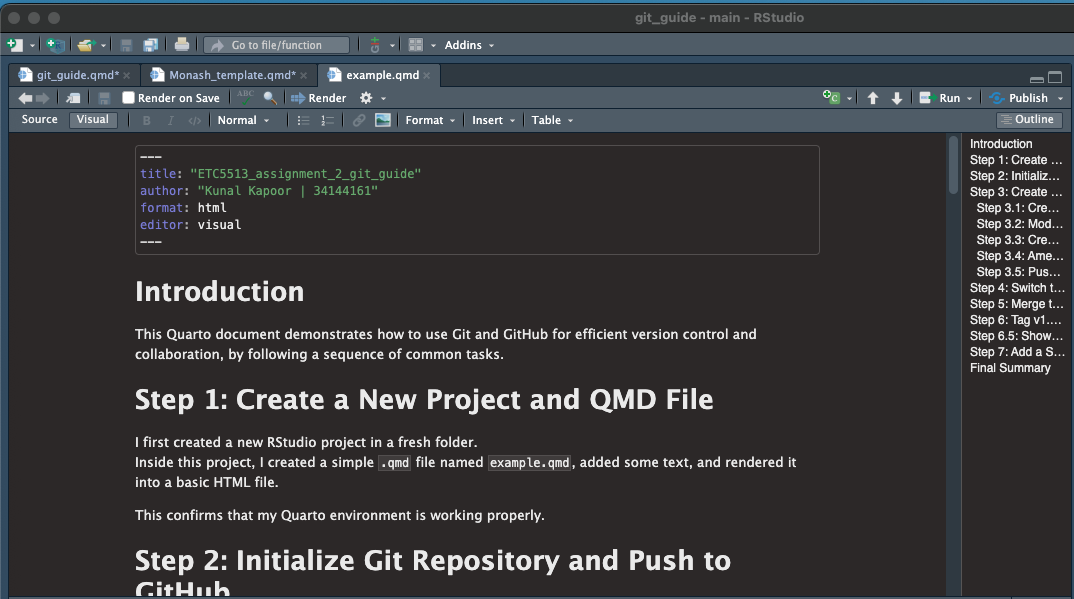
\includegraphics[keepaspectratio]{images/rstudio_working.png}}

}

\caption{File in Rstudio environment}

\end{figure}%%
\begin{figure}[H]

{\centering \pandocbounded{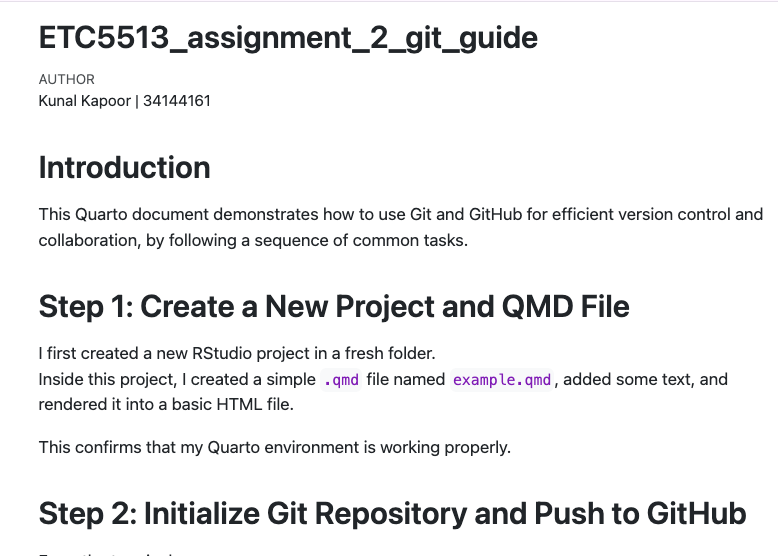
\includegraphics[keepaspectratio]{images/rendered_html.png}}

}

\caption{HTML Render in Web Browser}

\end{figure}%

\newpage

\subsubsection{Step 2: Let's make our first
commit}\label{step-2-lets-make-our-first-commit}

Now that we have our example.qmd and the rendered HTML file, it's time
to save a snapshot of our project using Git.

This snapshot is called a commit.

Think of a commit like saving a version of your project at a particular
moment ---so if something goes wrong later, you can always rewind back
to this point!

\subsubsection{Step 2.1: Stage your
work}\label{step-2.1-stage-your-work}

First we check which files Git is already tracking by running a simple
command in our command line interface {[} Guess what can tell us the
status of GIT? {]}

\begin{verbatim}
git status 
\end{verbatim}

This shows you which files Git is tracking and which ones are new.

You should see something like:

\begin{verbatim}
Untracked files:
  (use "git add <file>..." to include in what will be committed)
    example.qmd
    example.html
\end{verbatim}

These are files Git knows exist but hasn't saved yet.

\begin{itemize}
\tightlist
\item
  To stage them (prepare them for committing), run:
\end{itemize}

\begin{verbatim}
git add example.qmd 
\end{verbatim}

This creates the first checkpoint of our project and also tell Git:

\emph{``Hey, I want to include these files in the next snapshot.''}

\subsubsection{Step 2.2: Save (Commit) your
Snapshot}\label{step-2.2-save-commit-your-snapshot}

Now that the files are staged, let's commit them:

\begin{verbatim}
git commit -m "First Commit - Added example.qmd and rendered HTML files"
\end{verbatim}

The \textbf{-m} lets you attach a short message describing what this
commit is about.

\begin{itemize}
\item
  Why This Step Matters:

  \begin{itemize}
  \item
    Staging ensures you're only saving what you really intend to.
  \item
    Commit messages are like breadcrumbs --- they help you (and your
    future teammates) understand what changes were made, and why.
  \end{itemize}
\end{itemize}

\begin{longtable}[]{@{}
  >{\raggedright\arraybackslash}p{(\linewidth - 2\tabcolsep) * \real{0.2222}}
  >{\raggedright\arraybackslash}p{(\linewidth - 2\tabcolsep) * \real{0.7500}}@{}}
\caption{Recap of step 2}\tabularnewline
\toprule\noalign{}
\begin{minipage}[b]{\linewidth}\raggedright
\textbf{STEP}
\end{minipage} & \begin{minipage}[b]{\linewidth}\raggedright
\textbf{PURPOSE}
\end{minipage} \\
\midrule\noalign{}
\endfirsthead
\toprule\noalign{}
\begin{minipage}[b]{\linewidth}\raggedright
\textbf{STEP}
\end{minipage} & \begin{minipage}[b]{\linewidth}\raggedright
\textbf{PURPOSE}
\end{minipage} \\
\midrule\noalign{}
\endhead
\bottomrule\noalign{}
\endlastfoot
\begin{minipage}[t]{\linewidth}\raggedright
\begin{verbatim}
git status
\end{verbatim}
\end{minipage} & Check what git is tracking \\
\begin{minipage}[t]{\linewidth}\raggedright
\begin{verbatim}
git add
\end{verbatim}
\end{minipage} & Prepare the files for commit \\
\begin{minipage}[t]{\linewidth}\raggedright
\begin{verbatim}
git commit
\end{verbatim}
\end{minipage} & Save a snapshot with a message \\
\end{longtable}

\newpage

\subsubsection{Step 3: Link to GitHub and Push it
Oneline}\label{step-3-link-to-github-and-push-it-oneline}

Saving work on your computer is good.

But what if your laptop crashes? Or you want to show your work to
others?

That's why we push our Git repository to GitHub a safe place on the
internet to store your project and collaborate with others.

\subsubsection{Step 3.1: Create a new repository on
GitHub}\label{step-3.1-create-a-new-repository-on-github}

Now we connect our local project to GitHub and upload it.

First, log in to GitHub and create a new empty repository.

\begin{verbatim}
•   Don’t initialize it with a README, .gitignore, or license.
\end{verbatim}

(Otherwise Git will get confused when pushing.)

Once created, GitHub will show you the repository URL --- something
like:

\begin{verbatim}
https://github.com/your-username/your-repository.git
\end{verbatim}

\emph{Copy this link --- we'll need it next!}

\subsubsection{Step 3.2: Connect Local project to GitHub (Remote
Link)}\label{step-3.2-connect-local-project-to-github-remote-link}

In your terminal (inside your project folder), run:

\begin{verbatim}
git remote add origin <your-repository-URL>
\end{verbatim}

Replace \textless your-repository-URL\textgreater{} with the link you
copied from GitHub.\\

\begin{itemize}
\item
  \textbf{What this does:}

  \begin{itemize}
  \item
    It tells Git:
  \item
    \emph{``Hey, this is the address where you will send (push) all my
    project snapshots.''}
  \end{itemize}
\end{itemize}

Bonus tip:\\
To double-check that the connection was made:

\begin{verbatim}
git remote -v 
\end{verbatim}

We should see an output like this:

\begin{verbatim}
origin  https://github.com/your-username/your-repository.git (fetch)
origin  https://github.com/your-username/your-repository.git (push)
\end{verbatim}

This shows that Git knows exactly where our project will live online

\subsubsection{Step 3.3: Push our work to
GitHub}\label{step-3.3-push-our-work-to-github}

Now's let's send (push) our local commits to GitHub:

\begin{verbatim}
git push -u origin main 
\end{verbatim}

The -u flag tells Git to remember that ``origin/main'' is the default
place to push changes next time.

\textbf{\emph{(So from now on, you can just type git push.)\\
}}

\begin{itemize}
\item
  \textbf{Why This Step Matters:}

  \begin{itemize}
  \item
    Your work is now backed up safely online.
  \item
    You can access it from anywhere --- just log into GitHub.
  \item
    You're ready to collaborate with others if needed!
  \end{itemize}
\end{itemize}

QUICK TIPS:

\begin{enumerate}
\def\labelenumi{\arabic{enumi}.}
\item
  \textbf{Push after every major work session} to avoid losing progress.
\item
  \textbf{Don't push unfinished or broken work} unless you're using a
  branch meant for testing.\\
\end{enumerate}

\begin{longtable}[]{@{}
  >{\raggedright\arraybackslash}p{(\linewidth - 2\tabcolsep) * \real{0.3061}}
  >{\raggedright\arraybackslash}p{(\linewidth - 2\tabcolsep) * \real{0.6939}}@{}}
\caption{Step 3 \textbar{} Summary Table}\tabularnewline
\toprule\noalign{}
\begin{minipage}[b]{\linewidth}\raggedright
STEP
\end{minipage} & \begin{minipage}[b]{\linewidth}\raggedright
PURPOSE
\end{minipage} \\
\midrule\noalign{}
\endfirsthead
\toprule\noalign{}
\begin{minipage}[b]{\linewidth}\raggedright
STEP
\end{minipage} & \begin{minipage}[b]{\linewidth}\raggedright
PURPOSE
\end{minipage} \\
\midrule\noalign{}
\endhead
\bottomrule\noalign{}
\endlastfoot
Create Repository on GitHub & Set up an online space for your project \\
\begin{minipage}[t]{\linewidth}\raggedright
\begin{verbatim}
git remote add origin <
your-repository-URL>
\end{verbatim}
\end{minipage} & Connect your local Git project to the GitHub
repository \\
\begin{minipage}[t]{\linewidth}\raggedright
\begin{verbatim}
git remote -v
\end{verbatim}
\end{minipage} & Confirm that Git knows where to push and fetch from \\
\begin{minipage}[t]{\linewidth}\raggedright
\begin{verbatim}
git push -u origin main
\end{verbatim}
\end{minipage} & Upload your local project history to GitHub and
remember the link \\
\end{longtable}

\newpage

\subsubsection{Step 4: Create a New Branch and Make
Changes}\label{step-4-create-a-new-branch-and-make-changes}

When working on a project, it is a good idea to experiment or make
changes without touching your main working version.

In Git, we do this by creating a branch.

A branch is like a safe testing ground where you can make updates, try
new features, or fix mistakes without affecting the original project.

\subsubsection{Step 4.1: Create and a New
Branch}\label{step-4.1-create-and-a-new-branch}

In our command line interface we will run

\begin{verbatim}
git branch testbranch
\end{verbatim}

This only creates the branch. It does not move you into it yet.NOTE:

\subsubsection{Step 4.2: Switch to a New
Branch}\label{step-4.2-switch-to-a-new-branch}

Now, we switch into the new branch we just created by using

\begin{verbatim}
git checkout testbranch
\end{verbatim}

After switching, you are now working inside testbranch.\\
Any changes you make will stay isolated from your main branch.

\textbf{SHORTCUT}

\begin{verbatim}
git checkout -b testbrach 
\end{verbatim}

If we run the above command then both creation of new branch and
switching to the new branch happens at the same time.

\subsubsection{Step 4.3: Make A change in the
Branch}\label{step-4.3-make-a-change-in-the-branch}

Now that we are inside the testbranch, let's make a small change to
practice working safely inside a branch.

To do this:

\begin{enumerate}
\def\labelenumi{\arabic{enumi}.}
\item
  In RStudio, go to the top menu and click

  \begin{itemize}
  \tightlist
  \item
    File → New File → Quarto Document.
  \end{itemize}
\item
  Name the new file example.qmd if it is not already.
\item
  Inside example.qmd, make a small change --- for example, add a new
  heading:
\item
  Save the file after making your changes.
\end{enumerate}

\subsubsection{Step 4.4: Stage and Commit the changes in the
Branch}\label{step-4.4-stage-and-commit-the-changes-in-the-branch}

Now that we have made a change inside example.qmd and saved it, we need
to tell Git that we are ready to save this new version into the project
history.

In Git, this happens in two small actions:

\begin{itemize}
\item
  Staging (preparing the change)
\item
  Committing (saving the change)
\end{itemize}

\subsubsection{Step 4.4.1: Stage the
file}\label{step-4.4.1-stage-the-file}

First, we need to stage the changed file. In your terminal, run:

\begin{verbatim}
git add example.qmd
\end{verbatim}

This command tells git: '\emph{Please include this updated file in the
next snapshot'}

\subsubsection{Step 4.4.2: Commit the
Change}\label{step-4.4.2-commit-the-change}

After staging, we can now commit the change

\begin{verbatim}
 git commit -m 'Updated the example.qmd file with changes made in testbranch'
\end{verbatim}

The -m option allows you to add a \textbf{commit message} describing
what this change is about.

\subsubsection{Step 4.5: Push the Branch to
GitHub}\label{step-4.5-push-the-branch-to-github}

Now that we have committed our changes locally inside the testbranch,
the next step is to upload this new branch to GitHub.

This way, the changes are safely backed up online, and anyone you
collaborate with can also see your work.

\subsubsection{Step 4.5.1: Push the
Branch}\label{step-4.5.1-push-the-branch}

In our command line interface we will run the follwing command:

\begin{verbatim}
git push origin main 
\end{verbatim}

What this command does

\begin{itemize}
\item
  git push send the local changes to GitHub
\item
  -u (or --- set upstream) tells GitHub to remember that this branch
  should push and pull from origin/testbranch automatically in the
  future.
\end{itemize}

\begin{longtable}[]{@{}
  >{\raggedright\arraybackslash}p{(\linewidth - 2\tabcolsep) * \real{0.3721}}
  >{\raggedright\arraybackslash}p{(\linewidth - 2\tabcolsep) * \real{0.6279}}@{}}
\caption{Summary of Step 4}\tabularnewline
\toprule\noalign{}
\begin{minipage}[b]{\linewidth}\raggedright
STEP
\end{minipage} & \begin{minipage}[b]{\linewidth}\raggedright
PURPOSE
\end{minipage} \\
\midrule\noalign{}
\endfirsthead
\toprule\noalign{}
\begin{minipage}[b]{\linewidth}\raggedright
STEP
\end{minipage} & \begin{minipage}[b]{\linewidth}\raggedright
PURPOSE
\end{minipage} \\
\midrule\noalign{}
\endhead
\bottomrule\noalign{}
\endlastfoot
\begin{minipage}[t]{\linewidth}\raggedright
\begin{verbatim}
git branch testbranch
\end{verbatim}
\end{minipage} & Create a new branch called \emph{testbranch} \\
\begin{minipage}[t]{\linewidth}\raggedright
\begin{verbatim}
git checkout testbranch
\end{verbatim}
\end{minipage} & Switch to working inside the new branch \\
Create or edit example.qmd & Make a safe change inside the testbranch \\
\begin{minipage}[t]{\linewidth}\raggedright
\begin{verbatim}
git add example.qmd
\end{verbatim}
\end{minipage} & Stage the modified file for saving \\
\begin{minipage}[t]{\linewidth}\raggedright
\begin{verbatim}
git commit =-m'YOUR MESSAGE'
\end{verbatim}
\end{minipage} & Save the staged changes into Git history \\
\begin{minipage}[t]{\linewidth}\raggedright
\begin{verbatim}
git push -u origin testbranch
\end{verbatim}
\end{minipage} & Upload the testbranch to GitHub and set up tracking \\
\end{longtable}

\newpage

\subsubsection{Step 5: Add Data Folder and Amend Previous
Commit}\label{step-5-add-data-folder-and-amend-previous-commit}

Sometimes after making a commit, you realize you forgot to include an
important file or folder.

Instead of making a new commit for small things, Git allows you to amend
the last commit and update it.

In this step, we will:

\begin{enumerate}
\def\labelenumi{\arabic{enumi}.}
\item
  Create a new folder
\item
  Add files into it
\item
  Update (amend) our previous commit to include the new data
\item
  Push the corrected commit to GitHub
\end{enumerate}

\subsubsection{Step 5.1: Create a Data
Folder}\label{step-5.1-create-a-data-folder}

First, inside your project directory, create a new folder called data.

If you are using your computer's file explorer, simply create a new
folder named data.

Or, from the command line, you can run:

\begin{verbatim}
 mkdir data
\end{verbatim}

Now, move your Assignment 1 files (or any sample files) into this data
folder manually.

\subsubsection{Step 5.2: Stage the New Data
Folder}\label{step-5.2-stage-the-new-data-folder}

After adding our files into the data folder, we will tell git about the
new content by staging it

\begin{verbatim}
 git add data/
\end{verbatim}

This command stages the entire folder and all the files inside it for
the next commit.

\textbf{data/} - Tells the git to track and stage the entire contents of
the data folder.

\subsubsection{Step 5.3: Amend the Last
Commit}\label{step-5.3-amend-the-last-commit}

Now, instead of creating a new commit just for the data folder, we will
update our previous commit to include it.

Run:

\begin{verbatim}
git commit --amend --no-edit
\end{verbatim}

The --no-edit flag means you will keep the original commit message, but
update the files included.

Your last commit now contains:

\begin{itemize}
\item
  The original changes (e.g., your example.qmd edits)
\item
  Plus the newly added data folder.
\end{itemize}

\subsubsection{Step 5.4: Push the Amended Commit to
GitHub}\label{step-5.4-push-the-amended-commit-to-github}

Since we changed the commit history, we need to force push the update to
GitHub.

\begin{verbatim}
git push --force
\end{verbatim}

This command tells GitHub to replace the old commit with the new,
updated one.

\begin{longtable}[]{@{}
  >{\raggedright\arraybackslash}p{(\linewidth - 2\tabcolsep) * \real{0.3780}}
  >{\raggedright\arraybackslash}p{(\linewidth - 2\tabcolsep) * \real{0.6220}}@{}}
\caption{Summary Step 5}\tabularnewline
\toprule\noalign{}
\begin{minipage}[b]{\linewidth}\raggedright
STEP
\end{minipage} & \begin{minipage}[b]{\linewidth}\raggedright
PURPOSE
\end{minipage} \\
\midrule\noalign{}
\endfirsthead
\toprule\noalign{}
\begin{minipage}[b]{\linewidth}\raggedright
STEP
\end{minipage} & \begin{minipage}[b]{\linewidth}\raggedright
PURPOSE
\end{minipage} \\
\midrule\noalign{}
\endhead
\bottomrule\noalign{}
\endlastfoot
\begin{minipage}[t]{\linewidth}\raggedright
\begin{verbatim}
mkdir data
\end{verbatim}
\end{minipage} & Create a new folder to strore project data \\
Moves files into data/ & Add Assignment 1 or example files \\
\begin{minipage}[t]{\linewidth}\raggedright
\begin{verbatim}
git add data/
\end{verbatim}
\end{minipage} & Stage the new folder and it's contents \\
\begin{minipage}[t]{\linewidth}\raggedright
\begin{verbatim}
git commit --amend --no-edit
\end{verbatim}
\end{minipage} & Update the last commit to include the new folder \\
\begin{minipage}[t]{\linewidth}\raggedright
\begin{verbatim}
git push --force
\end{verbatim}
\end{minipage} & Push the amended commit to GitHub \\
\end{longtable}

\newpage

\subsubsection{Step 6: Modify Main Branch to Create
Conflict}\label{step-6-modify-main-branch-to-create-conflict}

In real projects, when multiple people work on the same files, sometimes
conflicts happen.

A conflict occurs when Git cannot automatically decide which version of
a file is correct because two people (or two branches) have changed the
same part of the file differently.

In this step, we will deliberately create a conflict between main and
testbranch, so we can practice resolving it.

\subsubsection{Step 6.1: Switch back to the Main
Branch}\label{step-6.1-switch-back-to-the-main-branch}

First, we need to move back to the main branch to make a separate change
there, let's run

\begin{verbatim}
git checkout main
\end{verbatim}

This command switched our working environment from \emph{testbranch}
back to \emph{main.}

\subsubsection{Step 6.2: Edit the Same File
Differently}\label{step-6.2-edit-the-same-file-differently}

Now open the example.qmd file again. Change the same part of the file
that you edited in testbranch, but make the content different.

For example, you could replace the previous heading with a new line
like:

\begin{verbatim}
## Different change made in main branch
\end{verbatim}

Save the file after making the changes.

\subsubsection{Step 6.3: Stage and Commit the
Change}\label{step-6.3-stage-and-commit-the-change}

Now that we have made a conflcting change in the main branch, let's
stage and commit the change:

First stage the updated file:

\begin{verbatim}
git add example.qmd
\end{verbatim}

Then let's commit it:

\begin{verbatim}
git commit -m 'Create conflicting change in the main branch'
\end{verbatim}

This saves the new version inside the main branch's history.

\subsubsection{Step 6.4: Push the changes to
GitHub}\label{step-6.4-push-the-changes-to-github}

Finally, upload the new commit to GitHub:

\begin{verbatim}
git push
\end{verbatim}

Now both your main branch and your testbranch have different changes to
the same file --- this sets us up perfectly to experience and learn how
to resolve a conflict when merging.

\begin{longtable}[]{@{}
  >{\raggedright\arraybackslash}p{(\linewidth - 2\tabcolsep) * \real{0.3605}}
  >{\raggedright\arraybackslash}p{(\linewidth - 2\tabcolsep) * \real{0.6395}}@{}}
\caption{Summary step 6}\tabularnewline
\toprule\noalign{}
\begin{minipage}[b]{\linewidth}\raggedright
STEP
\end{minipage} & \begin{minipage}[b]{\linewidth}\raggedright
PURPOSE
\end{minipage} \\
\midrule\noalign{}
\endfirsthead
\toprule\noalign{}
\begin{minipage}[b]{\linewidth}\raggedright
STEP
\end{minipage} & \begin{minipage}[b]{\linewidth}\raggedright
PURPOSE
\end{minipage} \\
\midrule\noalign{}
\endhead
\bottomrule\noalign{}
\endlastfoot
\begin{minipage}[t]{\linewidth}\raggedright
\begin{verbatim}
git checkout main
\end{verbatim}
\end{minipage} & Switch back to the main branch \\
Edit example.qmd & Make a different change in the same part of the
file \\
\begin{minipage}[t]{\linewidth}\raggedright
\begin{verbatim}
git add example.qmd
\end{verbatim}
\end{minipage} & Stage the new change \\
\begin{minipage}[t]{\linewidth}\raggedright
\begin{verbatim}
git commit -m 'YOUR MESSAGE'
\end{verbatim}
\end{minipage} & Save the change into Git history \\
\begin{minipage}[t]{\linewidth}\raggedright
\begin{verbatim}
git push
\end{verbatim}
\end{minipage} & Upload the updated main branch to GitHub \\
\end{longtable}

\newpage

\subsubsection{Step 7: Merge Branches and Resolve
Conflict}\label{step-7-merge-branches-and-resolve-conflict}

Now that both main and testbranch have different changes to the same
file, it is time to merge the branches.

Since the changes overlap, Git will not be able to merge them
automatically --- it will ask you to manually resolve the conflict.

This is an important skill for working in real projects where multiple
people edit the same files.

\subsubsection{Step 7.1: Merge testbranch into
main}\label{step-7.1-merge-testbranch-into-main}

First, make sure you are still in the main branch.

Then, try to merge the testbranch into main:

\begin{verbatim}
git merge testbranch
\end{verbatim}

Git will attempt to combine the changes but will detect a conflict
because git does not know which change to keep and which change to
discard, so ti will show a conflict message.

\begin{verbatim}
Auto-merging example.qmd
CONFLICT (content): Merge conflict in example.qmd
Automatic merge failed; fix conflicts and then commit the result.
\end{verbatim}

\subsubsection{Step 7.2: Understand the
Conflict}\label{step-7.2-understand-the-conflict}

Open example.qmd in your editor.

Git will have inserted conflict markers inside the file, showing you the
two versions:

\begin{verbatim}
<<<<<<< HEAD
This is the version from the main branch.
=======
This is the version from the testbranch.
>>>>>>> testbranc
\end{verbatim}

\begin{itemize}
\item
  The section between
  \textless\textless\textless\textless\textless\textless\textless{} HEAD
  and ======= shows what is currently in main.
\item
  The section between ======= and
  \textgreater\textgreater\textgreater\textgreater\textgreater\textgreater\textgreater{}
  testbranch shows what is coming from testbranch.
\item
  Our job is to choose which changes to keep, or combine them, and then
  remove all the conflict markers.
\end{itemize}

\subsubsection{Step 7.3: Fix the
Conflict}\label{step-7.3-fix-the-conflict}

Decide what the final content should be.

We can either:

\begin{enumerate}
\def\labelenumi{\arabic{enumi}.}
\item
  Keep only the main branch version,
\item
  Keep only the testbranch version,
\item
  Combine both versions in a clean way.
\end{enumerate}

Example (after resolving):

\begin{verbatim}
## Combined final version after conflict resolution

This line includes updates from both branches.
\end{verbatim}

This is after fixing the conflict manually, and saving the file.

\subsubsection{Step 7.4: Stage and Commit the Resolved
file}\label{step-7.4-stage-and-commit-the-resolved-file}

Now, stage the resolved file:

\begin{verbatim}
git add example.qmd 
\end{verbatim}

Add the commit message

\begin{verbatim}
git commit -m 'Resolved the merge conflict manually between main and testbranch'
\end{verbatim}

This officially completes the merge.

\subsubsection{Step 7.5: Push the merged changes to
GitHub}\label{step-7.5-push-the-merged-changes-to-github}

Finally let's push all our changes to GitHub

\begin{verbatim}
git push
\end{verbatim}

Now our main branch on GitHub includes the merged content from both
branches.

\begin{longtable}[]{@{}
  >{\raggedright\arraybackslash}p{(\linewidth - 2\tabcolsep) * \real{0.4051}}
  >{\raggedright\arraybackslash}p{(\linewidth - 2\tabcolsep) * \real{0.5949}}@{}}
\caption{Summary Step 7}\tabularnewline
\toprule\noalign{}
\begin{minipage}[b]{\linewidth}\raggedright
STEP
\end{minipage} & \begin{minipage}[b]{\linewidth}\raggedright
PURPOSE
\end{minipage} \\
\midrule\noalign{}
\endfirsthead
\toprule\noalign{}
\begin{minipage}[b]{\linewidth}\raggedright
STEP
\end{minipage} & \begin{minipage}[b]{\linewidth}\raggedright
PURPOSE
\end{minipage} \\
\midrule\noalign{}
\endhead
\bottomrule\noalign{}
\endlastfoot
\begin{minipage}[t]{\linewidth}\raggedright
\begin{verbatim}
git merge testbranch
\end{verbatim}
\end{minipage} & Merge changes from testbranch into main \\
Resolve the conflict manually & Edit the file to remove the conflict
markers \\
\begin{minipage}[t]{\linewidth}\raggedright
\begin{verbatim}
git add example.qmd
\end{verbatim}
\end{minipage} & Stage the resolved file \\
\begin{minipage}[t]{\linewidth}\raggedright
\begin{verbatim}
git commit -m 'YOUR MESSAGE'
\end{verbatim}
\end{minipage} & Save the merged result \\
\begin{minipage}[t]{\linewidth}\raggedright
\begin{verbatim}
git push
\end{verbatim}
\end{minipage} & Upload the merged branch to GitHub \\
\end{longtable}

\newpage

\subsubsection{Step 8: Tagging a
Version}\label{step-8-tagging-a-version}

When working on a project, it is useful to mark important milestones for
example, when you complete a feature, fix a major bug, or reach a stable
release.

In Git, you can tag a specific commit with a label to make it easy to
find later. Tags are often used to mark official version releases like
v1.0, v2.0, and so on.

In this step, we will tag our project as version v1.0 after successfully
merging the branches.

\textbf{Step 8.1: Create an Annotated Tag}

In your terminal, run the following command:

\begin{verbatim}
git tag - a v1.0 -m 'Version 1.0 release'
\end{verbatim}

\textbf{Explanation:}

\begin{itemize}
\item
  -a v1.0 creates an annotated tag named v1.0.
\item
  -m ``\ldots{}'' provides a short message describing the tag.
\end{itemize}

Annotated tags store important information like:

\begin{enumerate}
\def\labelenumi{\arabic{enumi}.}
\item
  Tag name
\item
  Tag message
\item
  Tagger's name
\item
  Date and time
\end{enumerate}

This makes it more useful than a simple lightweight tag.

\subsubsection{Step 8.2: Push the Tag to
GitHub}\label{sec-step-8.2-push-the-tag-to-github}

By default, tags are not automatically pushed when you run git push and
we must push them separately.

Push the tag using:

\begin{verbatim}
git push origin v1.0 
\end{verbatim}

This command sends your tag to GitHub, so it is stored along with your
project. Now anyone who views your repository can see that version v1.0
has been marked

\begin{longtable}[]{@{}
  >{\raggedright\arraybackslash}p{(\linewidth - 2\tabcolsep) * \real{0.3253}}
  >{\raggedright\arraybackslash}p{(\linewidth - 2\tabcolsep) * \real{0.6747}}@{}}
\caption{Summary step 8}\tabularnewline
\toprule\noalign{}
\begin{minipage}[b]{\linewidth}\raggedright
STEP
\end{minipage} & \begin{minipage}[b]{\linewidth}\raggedright
PURPOSE
\end{minipage} \\
\midrule\noalign{}
\endfirsthead
\toprule\noalign{}
\begin{minipage}[b]{\linewidth}\raggedright
STEP
\end{minipage} & \begin{minipage}[b]{\linewidth}\raggedright
PURPOSE
\end{minipage} \\
\midrule\noalign{}
\endhead
\bottomrule\noalign{}
\endlastfoot
\begin{minipage}[t]{\linewidth}\raggedright
\begin{verbatim}
git tag -a v1.0
-m "Version 1.0 release"
\end{verbatim}
\end{minipage} & Create an annotated tag for the current project
state \\
\begin{minipage}[t]{\linewidth}\raggedright
\begin{verbatim}
git push origin v1.0
\end{verbatim}
\end{minipage} & Upload the tag to GitHub \\
\end{longtable}

\newpage

\subsubsection{Step 9: Show Commit Log in Condensed
Form}\label{step-9-show-commit-log-in-condensed-form}

As you continue working with Git, your project history will grow with
many commits over time.

It can sometimes become difficult to quickly understand what has been
done without scrolling through long commit messages.

Git allows you to view the commit history in a condensed and
easy-to-read format, listing just short summaries.

In this step, we will view the condensed commit log.

\textbf{Step 9.1: View a Condensed Commit Log}

In your terminal, run:

\begin{verbatim}
git log --oneline
# Shows a compact list of all commits
\end{verbatim}

\textbf{What this does:}

\begin{itemize}
\item
  Shows each commit on a single line.
\item
  Displays the commit ID (shortened) and the commit message.
\end{itemize}

Example output:

\begin{figure}[H]

{\centering \pandocbounded{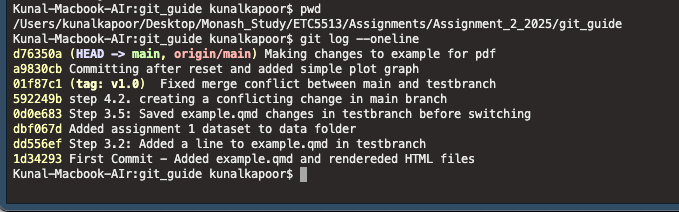
\includegraphics[keepaspectratio]{images/git_log_screenshot-min.png}}

}

\caption{Git log --oneline condensed form}

\end{figure}%

\begin{longtable}[]{@{}
  >{\raggedright\arraybackslash}p{(\linewidth - 2\tabcolsep) * \real{0.2778}}
  >{\raggedright\arraybackslash}p{(\linewidth - 2\tabcolsep) * \real{0.7222}}@{}}
\toprule\noalign{}
\begin{minipage}[b]{\linewidth}\raggedright
STEP
\end{minipage} & \begin{minipage}[b]{\linewidth}\raggedright
PURPOSE
\end{minipage} \\
\midrule\noalign{}
\endhead
\bottomrule\noalign{}
\endlastfoot
\begin{minipage}[t]{\linewidth}\raggedright
\begin{verbatim}
git log --oneline
\end{verbatim}
\end{minipage} & View a simplified one line summary of all commits \\
\end{longtable}

\newpage

\subsubsection{Step 10: Clean Up Old
Branch}\label{step-10-clean-up-old-branch}

Once you have successfully merged your changes from a branch into the
main project,

it is good practice to delete the branch if it is no longer needed.

This helps keep your repository organized and avoids confusion later.

In this step, we will delete the testbranch both locally (on your
computer) and remotely (on GitHub).

\textbf{Step 10.1: Delete the Branch Locally}

First, delete the branch from your local machine.

In your terminal, run:

\begin{verbatim}
git branch -d testbranch
\end{verbatim}

\textbf{What this does:}

\begin{itemize}
\item
  -d stands for ``delete''.
\item
  It safely deletes the branch, but only if it has already been merged.
\item
  Git will prevent you from deleting unmerged branches unless you force
  it.
\end{itemize}

If you see an error that says the branch is not fully merged, and you
still want to delete it (not recommended unless you are sure), you could
use:

\begin{verbatim}
git branch -D testbranch
\end{verbatim}

(But for our case, we use -d because we merged it correctly.)

\subsubsection{Step 10.2: Delete the Branch
Remotely}\label{step-10.2-delete-the-branch-remotely}

Now, delete the branch from GitHub as well.

Run:

\begin{verbatim}
git push origin --delete testbranch 
\end{verbatim}

What this does:

\begin{itemize}
\item
  origin is the name of your remote repository on GitHub.
\item
  --delete testbranch tells Git to remove the testbranch from GitHub.
\end{itemize}

After this, testbranch will no longer appear in the list of branches on
GitHub.

\begin{longtable}[]{@{}
  >{\raggedright\arraybackslash}p{(\linewidth - 2\tabcolsep) * \real{0.3750}}
  >{\raggedright\arraybackslash}p{(\linewidth - 2\tabcolsep) * \real{0.5972}}@{}}
\caption{Summary Step 10}\tabularnewline
\toprule\noalign{}
\begin{minipage}[b]{\linewidth}\raggedright
STEP
\end{minipage} & \begin{minipage}[b]{\linewidth}\raggedright
PURPOSE
\end{minipage} \\
\midrule\noalign{}
\endfirsthead
\toprule\noalign{}
\begin{minipage}[b]{\linewidth}\raggedright
STEP
\end{minipage} & \begin{minipage}[b]{\linewidth}\raggedright
PURPOSE
\end{minipage} \\
\midrule\noalign{}
\endhead
\bottomrule\noalign{}
\endlastfoot
\begin{minipage}[t]{\linewidth}\raggedright
\begin{verbatim}
git branch -d testbranch
\end{verbatim}
\end{minipage} & Delete the local testbranch after merge \\
\begin{minipage}[t]{\linewidth}\raggedright
\begin{verbatim}
git push origin
--delete testbranch
\end{verbatim}
\end{minipage} & Delete the remote testbranch from GitHub \\
\end{longtable}

\newpage

\subsubsection{Step 11: Undo a Commit (Without Losing
Changes)}\label{step-11-undo-a-commit-without-losing-changes}

Sometimes, you might commit your changes too early ---

maybe you forgot to edit something, or you want to improve your commit
message.

In Git, you can undo the last commit while keeping all your file changes
safe.

This is very useful when you want to fix your work without losing
anything.

\subsubsection{Step 11.1: Reset the last Commit
Softly:}\label{step-11.1-reset-the-last-commit-softly}

To undo the last commit but keep all your changes exactly as they were,
use the following command:

\begin{verbatim}
git reset --soft HEAD~1
\end{verbatim}

\textbf{What this command does:}

\begin{itemize}
\item
  reset moves the Git history back one step.
\item
  --soft keeps your files and staged changes exactly as they were.
\item
  HEAD\textasciitilde1 means ``one commit before the current one.''
\end{itemize}

After running this, your changes are still there --- they are just
uncommitted, waiting to be committed again (correctly this time).

\subsubsection{Step 11.2: Make any edits if
needed}\label{step-11.2-make-any-edits-if-needed}

At this point, you can:

\begin{itemize}
\item
  Edit your files if you want to make more changes.
\item
  Or, if everything is fine, just recommit with a better message.
\end{itemize}

\subsubsection{Step 11.3: Recommit
Properly}\label{step-11.3-recommit-properly}

When you are ready, you can stage (if needed) and commit again with a
better or corrected message:

\begin{verbatim}
git commit -m 'Updated section to include correct plot example'
\end{verbatim}

Now you have replaced the rushed commit with a better one --- and your
work is clean.

\begin{longtable}[]{@{}
  >{\raggedright\arraybackslash}p{(\linewidth - 2\tabcolsep) * \real{0.3421}}
  >{\raggedright\arraybackslash}p{(\linewidth - 2\tabcolsep) * \real{0.6579}}@{}}
\caption{Summary step 11}\tabularnewline
\toprule\noalign{}
\begin{minipage}[b]{\linewidth}\raggedright
STEP
\end{minipage} & \begin{minipage}[b]{\linewidth}\raggedright
PURPOSE
\end{minipage} \\
\midrule\noalign{}
\endfirsthead
\toprule\noalign{}
\begin{minipage}[b]{\linewidth}\raggedright
STEP
\end{minipage} & \begin{minipage}[b]{\linewidth}\raggedright
PURPOSE
\end{minipage} \\
\midrule\noalign{}
\endhead
\bottomrule\noalign{}
\endlastfoot
\begin{minipage}[t]{\linewidth}\raggedright
\begin{verbatim}
git reset --soft HEAD~1
\end{verbatim}
\end{minipage} & Undo the last commit but keep all local changes \\
Edit and Recommit & Fix mistakes and save a cleaner commit \\
\end{longtable}

The last commit is undone, but your edits remain staged, ready for a
better commit. \newpage

\section{Summary of Actions}\label{summary-of-actions}

By following these steps, you learned how to:

\begin{itemize}
\item
  Set up a Git repository
\item
  Track and save changes
\item
  Work safely using branches
\item
  Connect your project to a remote GitHub repository
\item
  Push and pull changes to/from GitHub
\item
  Handle merge conflicts
\item
  Tag versions
\item
  Manage commits and undo mistakes \newpage
\end{itemize}

\section{Git Commands Quick
Reference}\label{git-commands-quick-reference}

\begin{longtable}[]{@{}
  >{\raggedright\arraybackslash}p{(\linewidth - 4\tabcolsep) * \real{0.2831}}
  >{\raggedright\arraybackslash}p{(\linewidth - 4\tabcolsep) * \real{0.4398}}
  >{\raggedright\arraybackslash}p{(\linewidth - 4\tabcolsep) * \real{0.2711}}@{}}
\caption{Quick reference table summarizing important Git commands and
their purposes.}\tabularnewline
\toprule\noalign{}
\begin{minipage}[b]{\linewidth}\raggedright
\ul{\textbf{Git Command}}
\end{minipage} & \begin{minipage}[b]{\linewidth}\raggedright
\ul{\textbf{Meaning}}
\end{minipage} & \begin{minipage}[b]{\linewidth}\raggedright
\ul{\textbf{Why It's Useful}}
\end{minipage} \\
\midrule\noalign{}
\endfirsthead
\toprule\noalign{}
\begin{minipage}[b]{\linewidth}\raggedright
\ul{\textbf{Git Command}}
\end{minipage} & \begin{minipage}[b]{\linewidth}\raggedright
\ul{\textbf{Meaning}}
\end{minipage} & \begin{minipage}[b]{\linewidth}\raggedright
\ul{\textbf{Why It's Useful}}
\end{minipage} \\
\midrule\noalign{}
\endhead
\bottomrule\noalign{}
\endlastfoot
\texttt{git\ init} & Start tracking the project with Git & Begin version
control \\
\texttt{git\ status} & Check the status of changes & See staged,
unstaged, or untracked files \\
\texttt{git\ add\ filename} & Stage a specific file & Prepare file for
committing \\
\texttt{git\ add\ .} & Stage all changes in the working directory &
Quickly add everything for commit \\
\texttt{git\ commit\ -m\ "message"} & Save a snapshot of changes &
Record work into Git history \\
\texttt{git\ log} & Show commit history & View detailed list of
commits \\
\texttt{git\ log\ -\/-oneline} & Condensed commit history & View a brief
summary of commits \\
\texttt{git\ branch} & List all branches & Manage and view project
branches \\
\texttt{git\ branch\ branch\_name} & Create a new branch & Work
separately without affecting the main \\
\texttt{git\ switch\ branch\_name} & Switch to another branch & Move
between versions \\
\texttt{git\ switch\ -c\ branch\_name} & Create and switch to a new
branch & Shortcut to save time \\
\texttt{git\ merge\ branch\_name} & Merge another branch into current &
Combine features safely \\
\texttt{git\ push} & Upload commits to GitHub & Share work online \\
\texttt{git\ push\ -u\ origin\ main} & Push and track a new branch & Set
up branch tracking \\
\texttt{git\ pull} & Download and merge remote changes & Stay updated
with remote \\
\texttt{git\ tag\ -a\ v1.0\ -m\ "message"} & Create an annotated tag &
Mark important project points \\
\texttt{git\ reset\ -\/-soft\ HEAD\textasciitilde{}1} & Undo last commit
but keep changes staged & Correct mistakes without losing work \\
\texttt{git\ remote\ add\ origin\ url} & Connect local repo to GitHub &
Set up a remote repository \\
\texttt{git\ remote\ -v} & View remote connections & Confirm remote
links \\
\texttt{git\ remote\ remove\ origin} & Remove a GitHub link & Disconnect
remote repository \\
\texttt{git\ branch\ -d\ branch\_name} & Delete a local branch & Clean
up after merging \\
\texttt{git\ stash} & Temporarily save uncommitted work & Save work
without committing \\
\texttt{git\ stash\ pop} & Reapply stashed work & Restore work and
continue \\
\texttt{git\ revert\ commit\_id} & Undo a specific commit safely & Safe
undo for public history \\
\texttt{git\ rebase\ branch\_name} & Move branch commits onto another
branch & Simplify commit history \\
\texttt{git\ rebase\ -i\ HEAD\textasciitilde{}n}(squash inside rebase) &
Interactive rebase to squash commits Combine multiple commits into one &
\begin{minipage}[t]{\linewidth}\raggedright
Clean multiple commits\\
Tidy commit history\strut
\end{minipage} \\
\end{longtable}

\section{Conclusion}\label{conclusion}

Mastering Git provides a strong foundation for any collaborative or
individual project work. Whether you are coding, writing, or analyzing
data, Git ensures that your progress is organized, secure, and easy to
manage.


\printbibliography



\end{document}
